\documentclass[../main.tex]{subfiles}
\graphicspath{{\subfix{../images/}}}
\begin{document}


\subsection{Uspořádání minimalizující zaplnění}

Optimální by bylo najít permutovanou matici $$\tilde{\mathbb{P}}, |Struct(L_{\tilde{\mathbb{P}} \mathbb{A} \tilde{\mathbb{P}}^T}) = \min_{Permutace} |Struct(L_{\mathbb{P}\mathbb{A}\mathbb{P}^T})|$$

Na toto není znám účinný algoritmus, pro nesymetrické matice je to NP-úplný problém.

Díky tomu hledáme "dostatečně dobrá" uspořádání, ne nutně optimální-

\subsubsection{Algoritmus minimálního stupně (Minimum degree ordering)}

\begin{enumerate}
    \item $G_0 = G(A), A_0 = A, i=1$
    \item V $G_{i}$ najdi vrchol s nejnižším stupněm a očísluj ho $\rightarrow i$
    \item Sestav $G_i$ eliminací $i$ z grafu $G_{i-1}$
    \item Dokud $i<n$, pak jdi na $2)$ jinak konec 
\end{enumerate}

Hlavní myšlenka algoritmu je, že vrcholy s malým stupněm způsobí malé zaplnění.

\begin{remark}
    Může se stát, že vrcholů s minimálním stupněm je více $\rightarrow$ různé verze algoritmu 
\end{remark}

\begin{remark}
    Algoritmus AMD (aproximate minimum degree) - stupně vrcholů se nepočítají přesně pouze se odhadují
\end{remark}

\subsection{Uspořádání přizpůsobující A počítačové architektuře}

\begin{figure}[H]
    \centering
    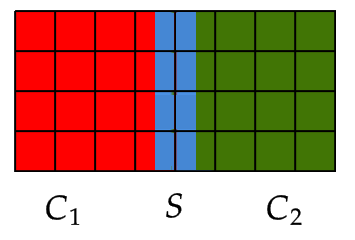
\includegraphics[width=0.5\linewidth]{images/2-11-usporadani.png}
    \caption*{S označuje takzvaný separátor}
\end{figure}

Rozdělím vrcholy v $G(A)$ na 2 komponenty (přibližně stejně velké) a separátor (malý).

Nejpve očíslujeme vrcholy  v $C_1$, pak v $C_2$ a nakonec v $S$

Matice pak vypadá následovně:

\begin{figure}[H]
    \centering
    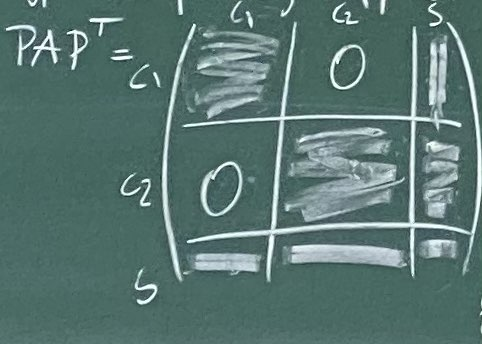
\includegraphics[width=0.5\linewidth]{images/2-11architekt.jpg}
\end{figure}

Ovroubený pásový tvar. 

Nulové bloky zůstanou při Choleského faktorizaci zachovány 


Diagonální bloky lze faktorizovat paralelně .

Výhodné pokud komponenty jsou velké a separátor malý.

Postup lze  rekurentně použít na $C_1$ a $C_2\rightarrow$ Metoda vnořených řezů (nested disection), viz obrázek.
\begin{figure}[H]
    \centering
    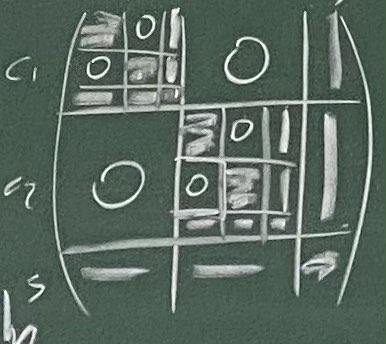
\includegraphics[width=0.5\linewidth]{images/2-11-nesteddissection.jpg}
\end{figure}

\subsubsection{Frontální metoda}

Uspořádání $A$ lze hledat za běhu Choleského faktorizace 

V každém kroku permutujeme řádky a sloupce matice \matA tak, aby se nenulové prvky nahrnuly k diagonále.

U pásových matic se eliminace provádí v malých hustých maticích, nic se nemusí přehazovat.
Tato metoda má nevýhodu, permuce za běhu je drahá. 
Její hlavní výhoda je možnost konstruovat Choleského rozklad matice \matA i když \matA není celá složená.

Toto má aplikaci v MKP, \matA se skládá z příspěvků jednotlivých elemntů, nemusí se skládad \matA , ale rovnou její Choleského rozklad.



\section{Poznámky k obecnějším systémum}

\subsection{Symetrické indefinitní matice}

\begin{example}
    \begin{equation*}        
        \mathbb{A} = \begin{pmatrix}
            0 & 1 \\
            1 & 0
        \end{pmatrix}
    \end{equation*}

    $a_{11}=0$, nelze dělit nulou a Choleského rozklad neexistuje.

    Je třeba permutovat řádky a sloupce matice \matA, ale žádnou symetrickou permutací nedostaneme $a_{11}\neq 0$.

    Při nesymetrické permutaci ztratíme symetrii - nebudeme diskutovat obecný indefinitní případ
\end{example}

Symetrické indefinitní soustavy vznikají například ve smíšené formulaci MKP nebo při řešené vázaných extrémů funkcí.

V tomto případě má matice \matA následující tvar:

\begin{equation*}
    \mathbb{R}^{n,m} \rightarrow \mathbb{A} = \begin{pmatrix}
        \mathbb{B} & \mathbb{C}\\
        \mathbb{C}^T & 0
    \end{pmatrix}
\end{equation*}
A dále pro $x\in \mathbb{R}^m, y \in \mathbb{R}^{n-m}$
\begin{equation}\label{eq:2-11:prvni}
    \mathbb{B} x + \mathbb{C} y = b_1
\end{equation}
\begin{equation}\label{eq:2-11:druha}
    \mathbb{C}^T x = b_2
\end{equation}

Obvykle navíc platí, že $\mathbb{B}\in \mathbb{R}^{m,m}$ je SPD a řídká, $\mathbb{C}\in\mathbb{R}^{m,m-n}, m\geq n-m$ a navíc $h(C) = n-m$.


Postup řešení je pak následující:

$\mathbb{B}$ je SPD $\implies\exists$ Choleského rozklad, tj. $\mathbb{B} = \mathbb{L}\mathbb{L}^T \implies$ máme $\mathbb{B}^{-1}$

Přenásobme \eqref{eq:2-11:prvni} $\mathbb{B}^{-1}$
\begin{equation*}
    x = \mathbb{B}^{-1} (b_1 - \mathbb{C}y)
\end{equation*}
dosadíme do \eqref{eq:2-11:druha}
\begin{equation*}
    \mathbb{C}^T \mathbb{B}^{-1} (b_1 - \mathbb{C}y) = b_2
\end{equation*}
Upravíme na 
\begin{equation*}
    \mathbb{C}^T \mathbb{B}^{-1} \mathbb{C} y = \mathbb{C}^T \mathbb{B}^{-1} b_1 - b_2 
\end{equation*}

Označme $\mathbb{C}^T \mathbb{B}^{-1} \mathbb{C} \eqcolon \mathbb{S} \in \mathbb{R}^{n-m, n-m}$, takzvaný Schurův doplněk.


Soustavu:
\begin{equation*}
    \mathbb{S} y = \mathbb{C}^T \mathbb{B}^{-1} b_1 - b_2 
\end{equation*}
lze řešit přímo nebo iterativně.


$\mathbb{B}$ je SPD a $h(C) = n-m \implies \mathbb{S}$ je SPD
\begin{equation*}
    <\mathbb{C}^T \mathbb{B}^{-1} \mathbb{C} y ,y> = <\mathbb{B}^{-1} \mathbb{C}y, \mathbb{C}y> \geq \alpha ||\mathbb{C}y||^2 > 0
\end{equation*}
, kde $\alpha$ je konstanta PD $\mathbb{B}^{-1}$.

$\mathbb{B}$ je SPD $\implies \mathbb{B}^{-1}$ je SPD $\Leftrightarrow y\neq 0$.


Nejprve budeme řešit $\mathbb{S} y = \mathbb{C}^T\mathbb{B}^{-1} b_1 - b_2 \rightarrow y $.
Pak řešíme $\mathbb{B} x = b_1 - \mathbb{C}_y$.

Obě soustavy mají $SPD$ matice. $\mathbb{S}$ je hustá (!), i když je $\mathbb{B}$ řídká.

Pokud je $n-m$ malá, pak hustota nevadí. Alternativně lze soustavu s maticí $\mathbb{S}$ řešit iteračně.
Pak není třeba $\mathbb{S}$ explicitně sestavovat, stačí s nimi umět přenásobovat vektory
\begin{equation*}
    \mathbb{S}y = \mathbb{C}^T\mathbb{B}^{-1}\mathbb{C} y = \mathbb{C}^T{\mathbb{L}^{-1}}^T \mathbb{L}^{-1} \mathbb{C} y
\end{equation*}

\begin{enumerate}
    \item Spočteme $\mathbb{C}y$
    \item Řešme $\mathbb{L} z = \mathbb{C}y \rightarrow z$
    \item $\mathbb{L}^T u = z$
    \item $\mathbb{S} y = \mathbb{C}^T u$ 
\end{enumerate}







\end{document}